\documentclass[sigconf]{acmart}

\usepackage{tikz}
\usetikzlibrary{arrows.meta,positioning}
\usepackage{algorithm}
\usepackage{algpseudocode}
\usepackage{booktabs}
\usepackage{xcolor}
\usepackage{url}
\usepackage{indentfirst}
\usepackage{xurl}
\usepackage{multirow}
\sloppy

% ACM boilerplate switched off / replaced by EDBT macros
\settopmatter{printacmref=false}
\renewcommand\footnotetextcopyrightpermission[1]{}
%% EDBT Conference Proceedings setup for ACM sigconf Style



%% EDBT: ISBN and year have to be adapted with every Number / Volume !
%%
\def\EDBTISSN{xxxx-xxxx}
\def\EDBTISBN{xxx-x-xxxxx-xxx-x}
\setcopyright{none}
\copyrightyear{\copyright\ 2027 Copyright held by the owner/author(s).
  Published on xxxxx under ISBN \EDBTISBN, series ISSN \EDBTISSN.
  Distribution of this paper is permitted under the terms of the
  Creative Commons license CC-by-nc-nd 4.0}
\acmYear{2027}
\acmDOI{}
\acmISBN{}


%% These commands are for a PROCEEDINGS abstract or paper.
%% EDBT: This needs adaptation every year!
\acmConference[EDBT '27]{Extending Database Technology}{6-9 April 2027}{Lille (France)}
%%
%%  Uncomment \acmBooktitle if the title of the proceedings is different
%%  from ``Proceedings of ...''!
%%
%%\acmBooktitle{Woodstock '18: ACM Symposium on Neural Gaze Detection,
%%  June 03--05, 2018, Woodstock, NY}


%% EDBT:
\settopmatter{printacmref=false, printccs=false, printfolios=false}


%% EDBT:
%% Macro to make image usable as hyperlink [see http://tex.stackexchange.com/questions/31819/xelatex-includegraphics-and-hyperlink]
\newsavebox{\ximagebox}
\newlength{\ximageheight}
\newsavebox{\xglyphbox}
\newlength{\xglyphheight}
\newcommand{\xbox}[1]%
  {\savebox{\ximagebox}{#1}%
  \settoheight{\ximageheight}{\usebox{\ximagebox}}%
  \savebox{\xglyphbox}{\color{white}\char32}%
  \settoheight{\xglyphheight}{\usebox{\xglyphbox}}%
  \raisebox{\ximageheight}[0pt][0pt]{\raisebox{-\xglyphheight}[0pt][0pt]{%
    \makebox[0pt][l]{\usebox{\xglyphbox}}}}%
    \usebox{\ximagebox}%
    \raisebox{0pt}[0pt][0pt]{\makebox[0pt][r]{\usebox{\xglyphbox}}}}

%% now use this to define the logo header:

\newsavebox{\LogoBox}
\sbox{\LogoBox}{}

%% now define our header and footer for the first page
\fancypagestyle{firstpagestyle}{%
  \fancyhf{}%
  \fancyfoot{}%
  \fancyhead[L,C]{}
  \fancyhead[R]{}{\raisebox{15pt}[0pt][0pt]{\xbox{\usebox{\LogoBox}}}}
  }

\hypersetup{%
  pdfcreator={LaTeX with acmart, hyperref, and EDBT modifications}
}

\settopmatter{printfolios=true}
\citestyle{acmnumeric}
\microtypesetup{expansion=false,protrusion=true}
\raggedbottom

\begin{document}

\title{Cascaded Semantic Joins over Structured and Unstructured Data}

\author{Anna Remizova, Sihem Amer-Yahia, Silviu Maniu}
\affiliation{%
  \institution{ CNRS, Univ. Grenoble Alpes}
  \city{Grenoble}
  \country{France}
}

\begin{abstract}
Questions that combine conditions on structured attributes (a movie's year or genre) with conditions on unstructured text (its reviews) require a large language model (LLM) as a semantic operator. \textsc{Suql} evaluates the semantic condition with one LLM call per candidate row, which is accurate but expensive; the semantic join of Trummer packs many rows into each call, which is cheaper but less accurate. We propose two cascaded architectures, \textsc{CasSuql} and \textsc{CasTrummer}, that run the structured filter in the DBMS, score the semantic condition with a cheap LLM, and escalate to an expensive LLM only the rows inside an ambiguity band. The band is calibrated with Beta-posterior credible bounds on the recall and precision of the cheap stage, estimated from a small score-stratified sample. On \textit{IMDb} and \textit{Amazon Fashion} (ten questions, ten repetitions each), the calibrated cascades lose no recall: \textsc{CasSuql} matches the F1 of \textsc{Suql} ($-0.2\%$, $+2.1\%$) while sending fewer rows to the expensive model. \textsc{CasTrummer} improves the F1 of \textsc{Trummer} by 110\% and 45\%, issues 81--83\% fewer LLM calls than \textsc{Suql}, and lies on the cost--F1 Pareto front on both datasets. An ablation attributes its quality gain to structural filtering and batched expensive verification, and a cost model states when the cheap stage itself saves time.
\end{abstract}

\keywords{LLM query processing, structured-unstructured query language, cascaded inference, semantic operators, cost-based optimization}

\maketitle
\thispagestyle{firstpagestyle}

\section{Introduction}
\label{sec:intro}

Consider the question \emph{``Which movies released in 1998 have reviews expressing an overall negative opinion?''} It needs (i) a structured filter over a \texttt{year} column and (ii) a semantic filter over free-text reviews. No structured query language can express the second half: a negative opinion has no fixed vocabulary (negation, sarcasm and implication all express it) and no schema to index it by. It therefore has to be delegated to a large language model (LLM) used as a query operator.

Two strategies exist. \textsc{Suql}~\cite{liu2023suql} compiles the structured half into SQL and calls the LLM once per surviving row, which gives high quality but a number of calls that grows with the candidates. Trummer~\cite{trummer2025semanticjoin} has the LLM join blocks of the two collections in one call, which needs far fewer calls but is less accurate, because one call must match rows, check the structured condition and judge the text. We build on both and add a cascade: a cheap stage scores each unit of work, and only units inside a calibrated ambiguity band reach the expensive stage. Our contributions, and what they buy, are:
\begin{itemize}
  \item \textbf{Calibrated cascades, \textsc{CasSuql} and \textsc{CasTrummer}.} Both run $\sigma_S$ in the DBMS first. The ambiguity band is derived from Beta-posterior credible bounds on the cheap stage's recall and precision, computed from 20 labeled rows stratified by cheap score, whose expensive answers are reused. A weak calibration can only cost money, never quality (\S\ref{sec:cascade-math}).
  \item \textbf{Quality with fewer calls.} \textsc{CasSuql} reproduces the quality of \textsc{Suql} while sending 5--14\% fewer rows to the expensive model, with no loss of recall. \textsc{CasTrummer} improves the F1 of \textsc{Trummer} by 110\% on \textit{IMDb} and 45\% on \textit{Amazon Fashion} with 28\% and 8\% fewer calls, issues 81--83\% fewer calls than \textsc{Suql}, and sits on the cost--F1 Pareto front of both datasets (\S\ref{sec:results}).
  \item \textbf{An explicit account of when the cascade pays off.} A cost model gives a break-even condition for the cheap stage, and an ablation separates the contribution of the cheap stage from that of structural filtering and batched verification (\S\ref{sec:cost}, \S\ref{sec:results}).
\end{itemize}
The rest of the paper reviews related work (\S\ref{sec:related}), the query model and baselines (\S\ref{sec:prelim}), the cascaded architectures and their calibration (\S\ref{sec:contributions}), and the experiments (\S\ref{sec:eval}).

\section{Related Work}
\label{sec:related}

\textbf{Avoiding LLM calls on rows a cheap check could reject.}
SUQL~\cite{liu2023suql} extends SQL with a free-text \texttt{answer()} function and shows that evaluating structured predicates before semantic ones is the dominant lever for controlling LLM cost, since it shrinks the candidate pool before the expensive operator. Our SUQL baseline follows this structure directly; our contribution is layering a cascade on top of the semantic operator itself, once filtering has already made the pool as small as it can.

\textbf{Avoiding one LLM call per row in the first place.} Trummer~\cite{trummer2025semanticjoin} treats semantic filtering as a block-nested-loops join: the LLM gets a batch of rows from each side at once and returns every match in a single call, with an adaptive batch size chosen to fit the model's context budget. Our Trummer baseline implements this algorithm directly; \textsc{CasTrummer} keeps its batching but adds structured filtering and calibrated escalation on top.

\textbf{Combining evidence from more than one source.}
ELEET~\cite{urban2024eleet} treats a semantic scan as a multi-modal operator, reading structured and unstructured evidence for the same entity from separate sources before selecting. It also gives a cost-aware reordering rule for a sequence of operators, which we reuse (\S\ref{sec:contributions}) to order the stages of \textsc{CasTrummer}.

\textbf{Deciding when a cheap stage can be trusted.} A hand-picked threshold gives no guarantee. Stretto~\cite{sanmartino2025stretto} calibrates a cheap stage with a Beta posterior over a log-odds score and adds a KV-cache-aware execution ladder; we build on the former, extended to a score-stratified sample (\S\ref{sec:cascade-math}), and skip the latter, which needs attention-state access our Ollama backend does not give. Other approaches calibrate on large validation sets with accuracy guarantees~\cite{zeighami2026bargain}, isotonic regression~\cite{kotte2026ucci}, learned proxy scores~\cite{zhang2025scaledoc} or learned routers~\cite{chen2023frugalgpt}; our setting must recalibrate for every question from a handful of labels.

\textbf{Classical query optimization.} Filtering ahead of an expensive operator goes back to cost-based join ordering~\cite{selinger1979access}, expensive-predicate scheduling~\cite{hellerstein1993predicate,hellerstein1998optimization,chaudhuri1996optimization} and the per-pair join cost it avoids~\cite{mishra1992join}. Text-to-SQL systems~\cite{gao2023textosql} handle only the structured half, a gap TAG~\cite{biswal2024tag} names explicitly; LOTUS~\cite{patel2024lotus} and Palimpzest~\cite{liu2024palimpzest} come closest to us, optimizing a full plan of declarative semantic operators with cost-based model choice and batching, whereas we optimize structured and unstructured predicates in tandem.

\section{Preliminaries}
\label{sec:prelim}

\textbf{Query model.} Let $S(\underline{\mathit{id}}, A_1,\dots,A_k)$ be a relation with structured attributes and $U(\mathit{id}, \mathit{txt})$ a relation of unstructured text. A question $Q = (\sigma_S,\sigma_U)$ has a structured predicate $\sigma_S$, answerable in a DBMS, and a semantic predicate $\sigma_U$ over $\mathit{txt}$, delegated to an LLM. Its answer is $\mathrm{Ans}(Q) := \pi_{\mathit{id}}\left(\sigma_S(S) \bowtie_{\mathit{id}} \sigma_U(U)\right)$. We assume the predicates are evaluated on disjoint evidence, so their selectivities are independent, and that $\sigma_S$ is far cheaper than $\sigma_U$: all methods try to spend as few LLM calls on $\sigma_U$ as possible. Predicate extraction, which maps a natural-language question to $(\sigma_S,\sigma_U)$, is a single LLM call shared by the four methods, which therefore differ only in how they compute $\mathrm{Ans}(Q)$.

\textbf{\textsc{Suql}.} $\sigma_S$ becomes a \texttt{WHERE} clause, yielding candidates $R_\sigma = \sigma_S(S)$; the LLM is called once per candidate through \texttt{answer(txt, question)}, for $O(|R_\sigma|)$ calls. Each row is judged alone with its full text, so quality is close to the best achievable, but the cost cannot be reduced because no work is shared across rows.

\textbf{\textsc{Trummer}.} No structured filter is applied. The two relations are partitioned into blocks and each call receives one block of each, like a block nested-loop join; the model must match rows by id, evaluate $\sigma_S$ without a query engine, and evaluate $\sigma_U$. This divides the number of calls by roughly the block size, but the three tasks in one call cost quality: the model tends to rely on the structured condition alone or on superficial keywords.

\begin{figure}[t]
\centering
\resizebox{\columnwidth}{!}{%
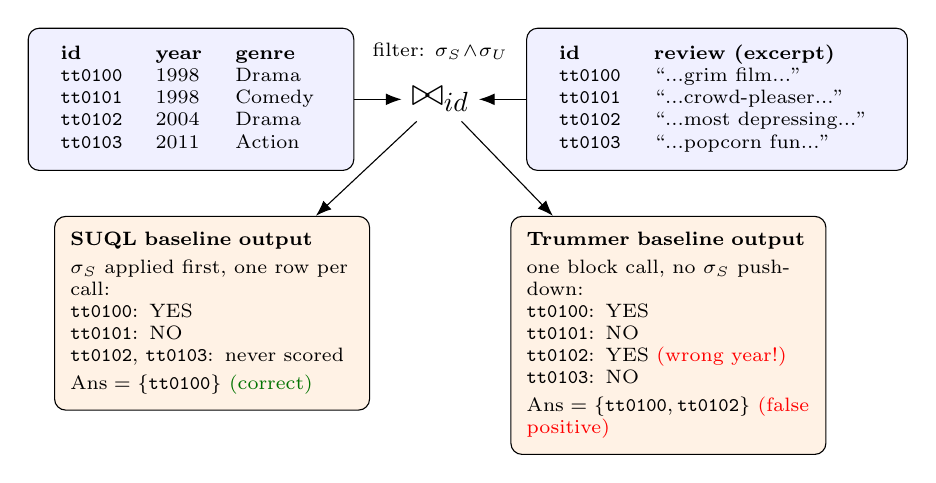
\begin{tikzpicture}[
  node distance=6mm and 6mm,
  tbl/.style={draw, rounded corners, align=left, font=\scriptsize, inner sep=2mm, fill=blue!6},
  outbox/.style={draw, rounded corners, align=left, font=\scriptsize, inner sep=2mm, fill=orange!10, text width=3.6cm},
  arr/.style={-{Latex[length=2mm]}}
]
\node[tbl] (R) {
  \begin{tabular}{lll}
    \textbf{id} & \textbf{year} & \textbf{genre}\\
    \texttt{tt0100} & 1998 & Drama\\
    \texttt{tt0101} & 1998 & Comedy\\
    \texttt{tt0102} & 2004 & Drama\\
    \texttt{tt0103} & 2011 & Action
  \end{tabular}
};
\node[font=\Large, right=6mm of R] (bowtie) {$\bowtie_{\text{id}}$};
\node[tbl, right=6mm of bowtie] (T) {
  \begin{tabular}{ll}
    \textbf{id} & \textbf{review (excerpt)}\\
    \texttt{tt0100} & ``...grim film...''\\
    \texttt{tt0101} & ``...crowd-pleaser...''\\
    \texttt{tt0102} & ``...most depressing...''\\
    \texttt{tt0103} & ``...popcorn fun...''
  \end{tabular}
};
\node[font=\scriptsize, above=1mm of bowtie] (q) {filter: $\sigma_S\!\wedge\!\sigma_U$};
\node[outbox, below left=12mm and 4mm of bowtie] (suqlout) {
  \textbf{SUQL baseline output}\\[2pt]
  $\sigma_S$ applied first, one row per call:\\
  \texttt{tt0100}: YES\\
  \texttt{tt0101}: NO\\
  \texttt{tt0102}, \texttt{tt0103}: never scored\\[2pt]
  $\mathrm{Ans} = \{\texttt{tt0100}\}$ \textcolor{green!45!black}{(correct)}
};
\node[outbox, below right=12mm and 4mm of bowtie] (trumout) {
  \textbf{Trummer baseline output}\\[2pt]
  one block call, no $\sigma_S$ pushdown:\\
  \texttt{tt0100}: YES\\
  \texttt{tt0101}: NO\\
  \texttt{tt0102}: YES \textcolor{red}{(wrong year!)}\\
  \texttt{tt0103}: NO\\[2pt]
  $\mathrm{Ans} = \{\texttt{tt0100},\texttt{tt0102}\}$ \textcolor{red}{(false positive)}
};
\draw[arr] (R) -- (bowtie);
\draw[arr] (T) -- (bowtie);
\draw[arr] (bowtie) -- (suqlout);
\draw[arr] (bowtie) -- (trumout);
\end{tikzpicture}
}
\caption{The running example as a join.}
\label{fig:example-join}
\end{figure}

\begin{example}[Running example]
\label{ex:running}
For the question above, Figure~\ref{fig:example-join} shows four movies joined with one review each, one per row category used in our benchmark (\S\ref{sec:setup}): \texttt{tt0100} (1998, ``grim film'') is a \emph{true positive}; \texttt{tt0101} (1998, ``crowd-pleaser'') satisfies $\sigma_S$ but not $\sigma_U$; \texttt{tt0102} (2004, ``most depressing'') satisfies only $\sigma_U$; \texttt{tt0103} (2011, ``popcorn fun'') satisfies neither. \textsc{Suql} applies $\sigma_S$ first and judges only \texttt{tt0100} and \texttt{tt0101}, so $\mathrm{Ans}=\{\texttt{tt0100}\}$. \textsc{Trummer} hands all four rows to one call, which must match rows, apply $\sigma_S$ and apply $\sigma_U$ at once; a model that tracks the sentiment but drops the year check also accepts \texttt{tt0102}, a false positive.
\end{example}

\section{Cascaded Architectures}
\label{sec:contributions}

Both cascades share the structure of Algorithm~\ref{alg:cascade}. The structured filter runs first in the DBMS. A \emph{cheap stage} then scores every surviving row with a log-odds $\ell = \log\frac{p}{1-p}$, a calibrated \emph{band} $(\tau_-,\tau_+)$ routes rows (accept if $\ell \ge \tau_+$, reject if $\ell \le \tau_-$), and an \emph{expensive stage} judges only the rows inside the band. A side of the band that calibration cannot certify is left open ($\tau_+{=}{+}\infty$ or $\tau_-{=}{-}\infty$), so no row is decided by a cheap stage that has not been shown reliable.

\begin{algorithm}[t]
\caption{Cascade (\textsc{CasSuql}: $B{=}B'{=}1$; \textsc{CasTrummer}: batches $B$, $B'$)}
\label{alg:cascade}
\begin{algorithmic}[1]
\Require rows $R_\sigma$ passing $\sigma_S$; batch sizes $B,B'$; calibration size $|C|$; target $Q^\ast$, level $\alpha$
\State score every row with $\mathrm{Cheap}$ in batches of $B$ $\to$ $\ell_r$
\State $C \gets$ $|C|$ rows stratified by $\ell$; $y_C \gets \mathrm{Expensive}(C)$ \Comment{labels are kept as final answers}
\State $(\tau_-,\tau_+) \gets \mathrm{FitBand}(\ell, y_C, Q^\ast, \alpha)$ \Comment{\S\ref{sec:cascade-math}}
\State $\mathrm{Ans} \gets \{r \in C: y_r{=}\texttt{YES}\} \cup \{r \notin C: \ell_r \ge \tau_+\}$
\For{batch $b \subset \{r \notin C : \tau_- < \ell_r < \tau_+\}$, $|b| \le B'$}
  \State $\mathrm{Ans} \gets \mathrm{Ans} \cup \{r \in b : \mathrm{Expensive}(b)_r = \texttt{YES}\}$ \Comment{split and retry if the answer is unusable}
\EndFor
\State \Return $\mathrm{Ans}$
\end{algorithmic}
\end{algorithm}

\textbf{\textsc{CasSuql}} scores each row in one single-token call. The log-odds come from the answer-token log-probabilities: we pool all \texttt{Yes}-like and all \texttt{No}-like spellings among the ten most likely first tokens. The calibration rows keep their expensive answer, so no row is judged twice, and \textsc{CasSuql} never issues more expensive calls than \textsc{Suql}.

\textbf{\textsc{CasTrummer}} changes three things in \textsc{Trummer}. (1) \emph{Structured filter:} $\sigma_S$ runs in the DBMS, so no context is spent on rows it rejects, and the false positive \texttt{tt0102} of the example can no longer be admitted. (2) \emph{Batched cheap pass:} one call per batch of $B$ rows returns \texttt{YES}, \texttt{NO} or \texttt{UNCERTAIN} per row (mapped to $\ell=+2,0,-2$); allowing \texttt{UNCERTAIN} sends rows with indirect evidence to the expensive stage instead of labeling them \texttt{NO}. In the example, \texttt{tt0101} is rejected and the sarcastic review of \texttt{tt0100} is escalated and accepted. (3) \emph{Batched expensive verification:} escalated rows are verified in batches of $B'$. If a batch's answer is unusable (the prompt overflowed the context and the model omitted row ids), it is split in two and each half retried, so no candidate is silently dropped; every retry counts as an expensive call.

Filtering with $\sigma_S$ first is the classical rule of ordering selections by ascending $c_i/(1-s_i)$~\cite{hellerstein1993predicate,urban2024eleet}: $\sigma_S$ is nearly free and selective.

\subsection{Cost Analysis}
\label{sec:cost}
We count LLM calls, which dominate the cost. Let $N=|S|$ and $|R_\sigma|=sN$. \textsc{Trummer} is a block nested-loop join~\cite{garcia2008database,ramakrishnan2003database} and issues $O(N^2/(b_Sb_U))$ calls whatever $s$ is. The other methods are linear in $sN$: \textsc{Suql} issues $sN$ calls, \textsc{CasSuql} $sN$ cheap and $O(e\,sN)$ expensive calls, and \textsc{CasTrummer} $O(sN/B)$ cheap and $O(e\,sN/B')$ expensive calls, where $e$ is the escalated fraction. Calibration calls are not extra, since the calibration rows keep their expensive answer. The cascade saves expensive calls on the fraction $d=1-e$ of rows the cheap stage decides alone. In wall-clock time, a row-wise cascade pays $t_c$ per row for the cheap call and $t_e$ for the escalated rows, against $t_e$ per row for \textsc{Suql}, so it is faster exactly when
\[ t_c / t_e < d. \]

\subsection{Calibrating the Cascade}
\label{sec:cascade-math}
For each question, $|C|$ candidates are labeled by the expensive LLM. The sample is stratified by cheap score: the candidates are cut into $K{=}4$ equal-count strata (equal scores never straddle a cut) and the labels are spread evenly over them.

\textbf{Beta-posterior bounds.} Let stratum $h$ have $N_h$ candidates, $n_h$ of them labeled, $y_h$ of those positive. With a uniform prior, Beta-Binomial conjugacy~\cite{gelman2013bayesian} gives the positive rate $\pi_h\sim\mathrm{Beta}(1{+}y_h,1{+}n_h{-}y_h)$. Labeled rows keep their answer, so only the $U_h=N_h-n_h$ unlabeled rows can be lost or wrongly accepted; their positives number $X_h\sim\mathrm{Bin}(U_h,\pi_h)$. Rejecting the $b$ lowest strata leaves a recall, relative to the expensive model, of
\[ \rho_b = 1-\frac{\sum_{h\le b}X_h}{Y+\sum_h X_h}, \]
with $Y=\sum_h y_h$, and accepting strata $h\ge t$ without verification has precision $\varpi_t=\sum_{h\ge t}X_h/\sum_{h\ge t}U_h$. We propagate the posteriors to both by Monte Carlo (2,000 draws) and take lower credible bounds at level $\alpha{=}0.9$: $\widehat r_\alpha(b)=Q_{1-\alpha}(\rho_b)$ and $\widehat p_\alpha(t)=Q_{1-\alpha}(\varpi_t)$, where $Q_q$ is the $q$-quantile. With one stratum and a uniform sample they reduce to the $\mathrm{Beta}(1{+}\mathit{TP},1{+}\mathit{FN})$ and $\mathrm{Beta}(1{+}\mathit{TP},1{+}\mathit{FP})$ bounds. The band rejects the largest prefix of strata and accepts the largest suffix that clear the target $Q^\ast$:
\begin{align*}
\tau_- &= \text{top score of stratum }\max\{b:\widehat r_\alpha(b)\ge Q^\ast\},\\
\tau_+ &= \text{lowest score of stratum }\min\{t:\widehat p_\alpha(t)\ge Q^\ast\}.
\end{align*}
Anything not certified is escalated.

\textbf{Target and power.} We use $Q^\ast{=}0.8$; $0.9$ cannot be certified from 20 labels, since a cheap stage correct on all 20 has a lower bound of only 0.896. In simulations (300 pools per configuration, 40 to 1,000 rows, 10--30\% positives, cheap-score AUC 0.76--0.96, $|C|\in\{20,40,100\}$; script in the artifact) the true recall reached $Q^\ast$ in at least 99\% of the trials with a certified reject region, against a target of 90\%. The price is modest power: with $|C|=20$ the cheap stage decides on its own 8--13\% of the rows (1\% with 10\% positives), 28--36\% with $|C|=40$, and 56\% of a 1,000-row pool needs $|C|=100$.

\section{Experiments}
\label{sec:eval}

\subsection{Setup}
\label{sec:setup}
\textbf{Data and questions.} \textit{IMDb}: 25k movies (title, director, year, runtime, genres) and one review each. \textit{Amazon Fashion}: 186k products and 882k reviews (2018 McAuley Lab release), a cross-domain check. Each dataset has ten questions (\texttt{10q}), each evaluated on its own pool of 100 items. On \textit{IMDb} a pool holds the four row kinds of Example~\ref{ex:running}: 12 answers, 28 rows satisfying only $\sigma_S$, 30 only $\sigma_U$ and 30 neither, so 40 rows pass $\sigma_S$. On \textit{Amazon Fashion} 50 products pass $\sigma_S$, 15 of them answers; the ten questions are a held-out set, disjoint from the smaller suites used during development. \textit{IMDb} questions combine one or two structured conditions (genre, year, runtime) with one semantic condition on the reviews; the ten questions span seven genres and range from direct cues (\emph{funny}) to abstract, paraphrase-prone ones (\emph{chemistry}, \emph{approval of a twist}). \textit{Amazon Fashion} questions restrict the product type through its title and ask about a property described in the reviews. Ground truth is the conjunction of $\sigma_S$ and hand-authored regular-expression patterns encoding the semantic condition; no LLM judges. Labels are therefore deterministic, but a correct paraphrase outside the patterns counts as a negative, so absolute F1 values are best read as comparisons between methods.

\textbf{Metrics, models, parameters.} Quality is precision, recall and F1 of the returned ids; cost is LLM calls (cheap and expensive), wall-clock time and dollars, from accelerator time at \$3/hour. We report the mean and standard deviation over the ten questions of the per-question mean of ten repetitions; as all calls are at temperature 0, repetitions differ only in the calibration sample. All methods use Gemma~4~e2b (cheap) and Gemma~4~26b (expensive), served by Ollama on one NVIDIA H200; the baselines use only the expensive model. \textsc{Suql} and \textsc{CasSuql} process one row per call; \textsc{CasTrummer} uses $B{=}8$ and $B'{=}32$, and \textsc{Trummer} the 4,096-token budget of its optimizer~\cite{trummer2025semanticjoin}. Both cascades use $|C|{=}20$, $K{=}4$, $\alpha{=}0.9$, $Q^\ast{=}0.8$. Cheap scores of \textsc{CasSuql} are read from Ollama's native log-probabilities (its OpenAI-compatible endpoint returns none). Reviews are truncated before entering a prompt: to 1,800 characters for the cheap stage of \textsc{CasSuql}, 3,500 for both stages of \textsc{CasTrummer}, 6,000 for the expensive stage of \textsc{CasSuql} and \textsc{Suql}, and 1,400 for \textsc{Trummer}; the same limits apply to \textit{Amazon Fashion}, whose reviews are much shorter (median 270 characters, against 1,115 on \textit{IMDb}). Code, suites, prompts and scripts: \url{https://github.com/AnnaRemi/SemanticCascadedLLMJoins}.

\begin{table*}[t]
\centering\scriptsize
\setlength{\tabcolsep}{3pt}
\begin{tabular}{l rrrrr rrrrr}
\toprule
 & \multicolumn{5}{c}{\textit{IMDb} \texttt{10q}} & \multicolumn{5}{c}{\textit{Amazon Fashion} \texttt{10q}} \\
\cmidrule(lr){2-6}\cmidrule(lr){7-11}
Metric & \textsc{Suql} & \textsc{CasSuql} & \textsc{Trummer} & \textsc{CasTrummer} & \textit{CasT$^{-}$} & \textsc{Suql} & \textsc{CasSuql} & \textsc{Trummer} & \textsc{CasTrummer} & \textit{CasT$^{-}$} \\
\midrule
Precision & 0.818 (0.213) & \textbf{0.830 (0.196)} & 0.620 (0.313) & 0.779 (0.186) & \textit{0.788 (0.230)} & 0.820 (0.115) & \textbf{0.839 (0.113)} & 0.565 (0.200) & 0.755 (0.285) & \textit{0.673 (0.252)} \\
Recall & 0.400 (0.207) & 0.400 (0.203) & 0.275 (0.193) & \textbf{0.708 (0.189)} & \textit{0.725 (0.208)} & \textbf{0.807 (0.254)} & \textbf{0.807 (0.234)} & 0.473 (0.260) & 0.647 (0.325) & \textit{0.633 (0.360)} \\
F1 & 0.501 (0.168) & 0.500 (0.153) & 0.340 (0.182) & \textbf{0.713 (0.131)} & \textit{0.723 (0.165)} & 0.779 (0.142) & \textbf{0.796 (0.133)} & 0.464 (0.187) & 0.673 (0.294) & \textit{0.621 (0.303)} \\
Wall time (s) & \textbf{24.7 (0.9)} & 47.0 (2.4) & 25.4 (2.6) & 25.7 (2.6) & \textit{22.3 (2.2)} & 29.0 (2.1) & 53.1 (2.9) & 24.0 (5.4) & \textbf{23.2 (8.4)} & \textit{21.4 (9.1)} \\
LLM calls & 40.0 (0.0) & 78.0 (2.8) & 10.5 (1.3) & \textbf{7.6 (0.7)} & \textit{9.0 (0.0)} & 49.4 (0.5) & 92.0 (3.7) & 9.0 (2.4) & \textbf{8.2 (3.0)} & \textit{9.0 (3.4)} \\
Cost (\$) & \textbf{0.0206 (0.0008)} & 0.0391 (0.0020) & 0.0212 (0.0022) & 0.0214 (0.0022) & \textit{0.0186 (0.0018)} & 0.0242 (0.0017) & 0.0442 (0.0024) & 0.0200 (0.0045) & \textbf{0.0193 (0.0070)} & \textit{0.0178 (0.0076)} \\
\bottomrule
\end{tabular}
\caption{Quality and cost per question, mean (std.\ dev.) over the 10 questions, 10 repetitions each. Bold: best of the four methods. \textit{CasT$^{-}$}: \textsc{CasTrummer} without the cheap stage ($|C|{=}0$, so it decides no row; ablation).}
\label{tab:results}
\end{table*}

\begin{table*}[t]
\centering\scriptsize
\setlength{\tabcolsep}{4pt}
\begin{tabular}{l rrrr rrrr}
\toprule
 & \multicolumn{4}{c}{\textit{IMDb} \texttt{10q}} & \multicolumn{4}{c}{\textit{Amazon Fashion} \texttt{10q}} \\
\cmidrule(lr){2-5}\cmidrule(lr){6-9}
F1 & \textsc{Suql} & \textsc{CasSuql} & \textsc{Trummer} & \textsc{CasTrummer} & \textsc{Suql} & \textsc{CasSuql} & \textsc{Trummer} & \textsc{CasTrummer} \\
\midrule
q1 & 0.59 & 0.50 & 0.15 & \textbf{0.82} & 0.57 & \textbf{0.64} & 0.21 & 0.32 \\
q2 & \textbf{0.71} & \textbf{0.71} & 0.55 & 0.62 & 0.85 & \textbf{0.93} & 0.43 & \textbf{0.93} \\
q3 & 0.29 & 0.29 & 0.13 & \textbf{0.83} & 0.61 & 0.61 & 0.43 & \textbf{0.67} \\
q4 & 0.47 & 0.47 & 0.57 & \textbf{0.92} & \textbf{0.94} & \textbf{0.94} & 0.79 & 0.90 \\
q5 & \textbf{0.80} & \textbf{0.80} & 0.22 & 0.74 & 0.61 & \textbf{0.67} & 0.32 & \textbf{0.67} \\
q6 & 0.45 & 0.45 & 0.15 & \textbf{0.55} & \textbf{0.91} & \textbf{0.91} & 0.61 & 0.80 \\
q7 & \textbf{0.59} & 0.50 & 0.38 & 0.56 & 0.73 & 0.77 & 0.51 & \textbf{0.78} \\
q8 & 0.40 & 0.40 & 0.25 & \textbf{0.83} & \textbf{0.85} & \textbf{0.85} & 0.57 & \textbf{0.85} \\
q9 & 0.38 & 0.38 & 0.59 & \textbf{0.63} & \textbf{0.79} & 0.71 & 0.19 & 0.00 \\
q10 & 0.33 & 0.50 & 0.40 & \textbf{0.64} & \textbf{0.94} & \textbf{0.94} & 0.58 & 0.83 \\
\bottomrule
\end{tabular}
\caption{F1 per question (mean of 10 repetitions); bold: best of the four methods on that question.}
\label{tab:perq}
\end{table*}

\subsection{Results}
\label{sec:results}

\begin{figure}[t]
\centering
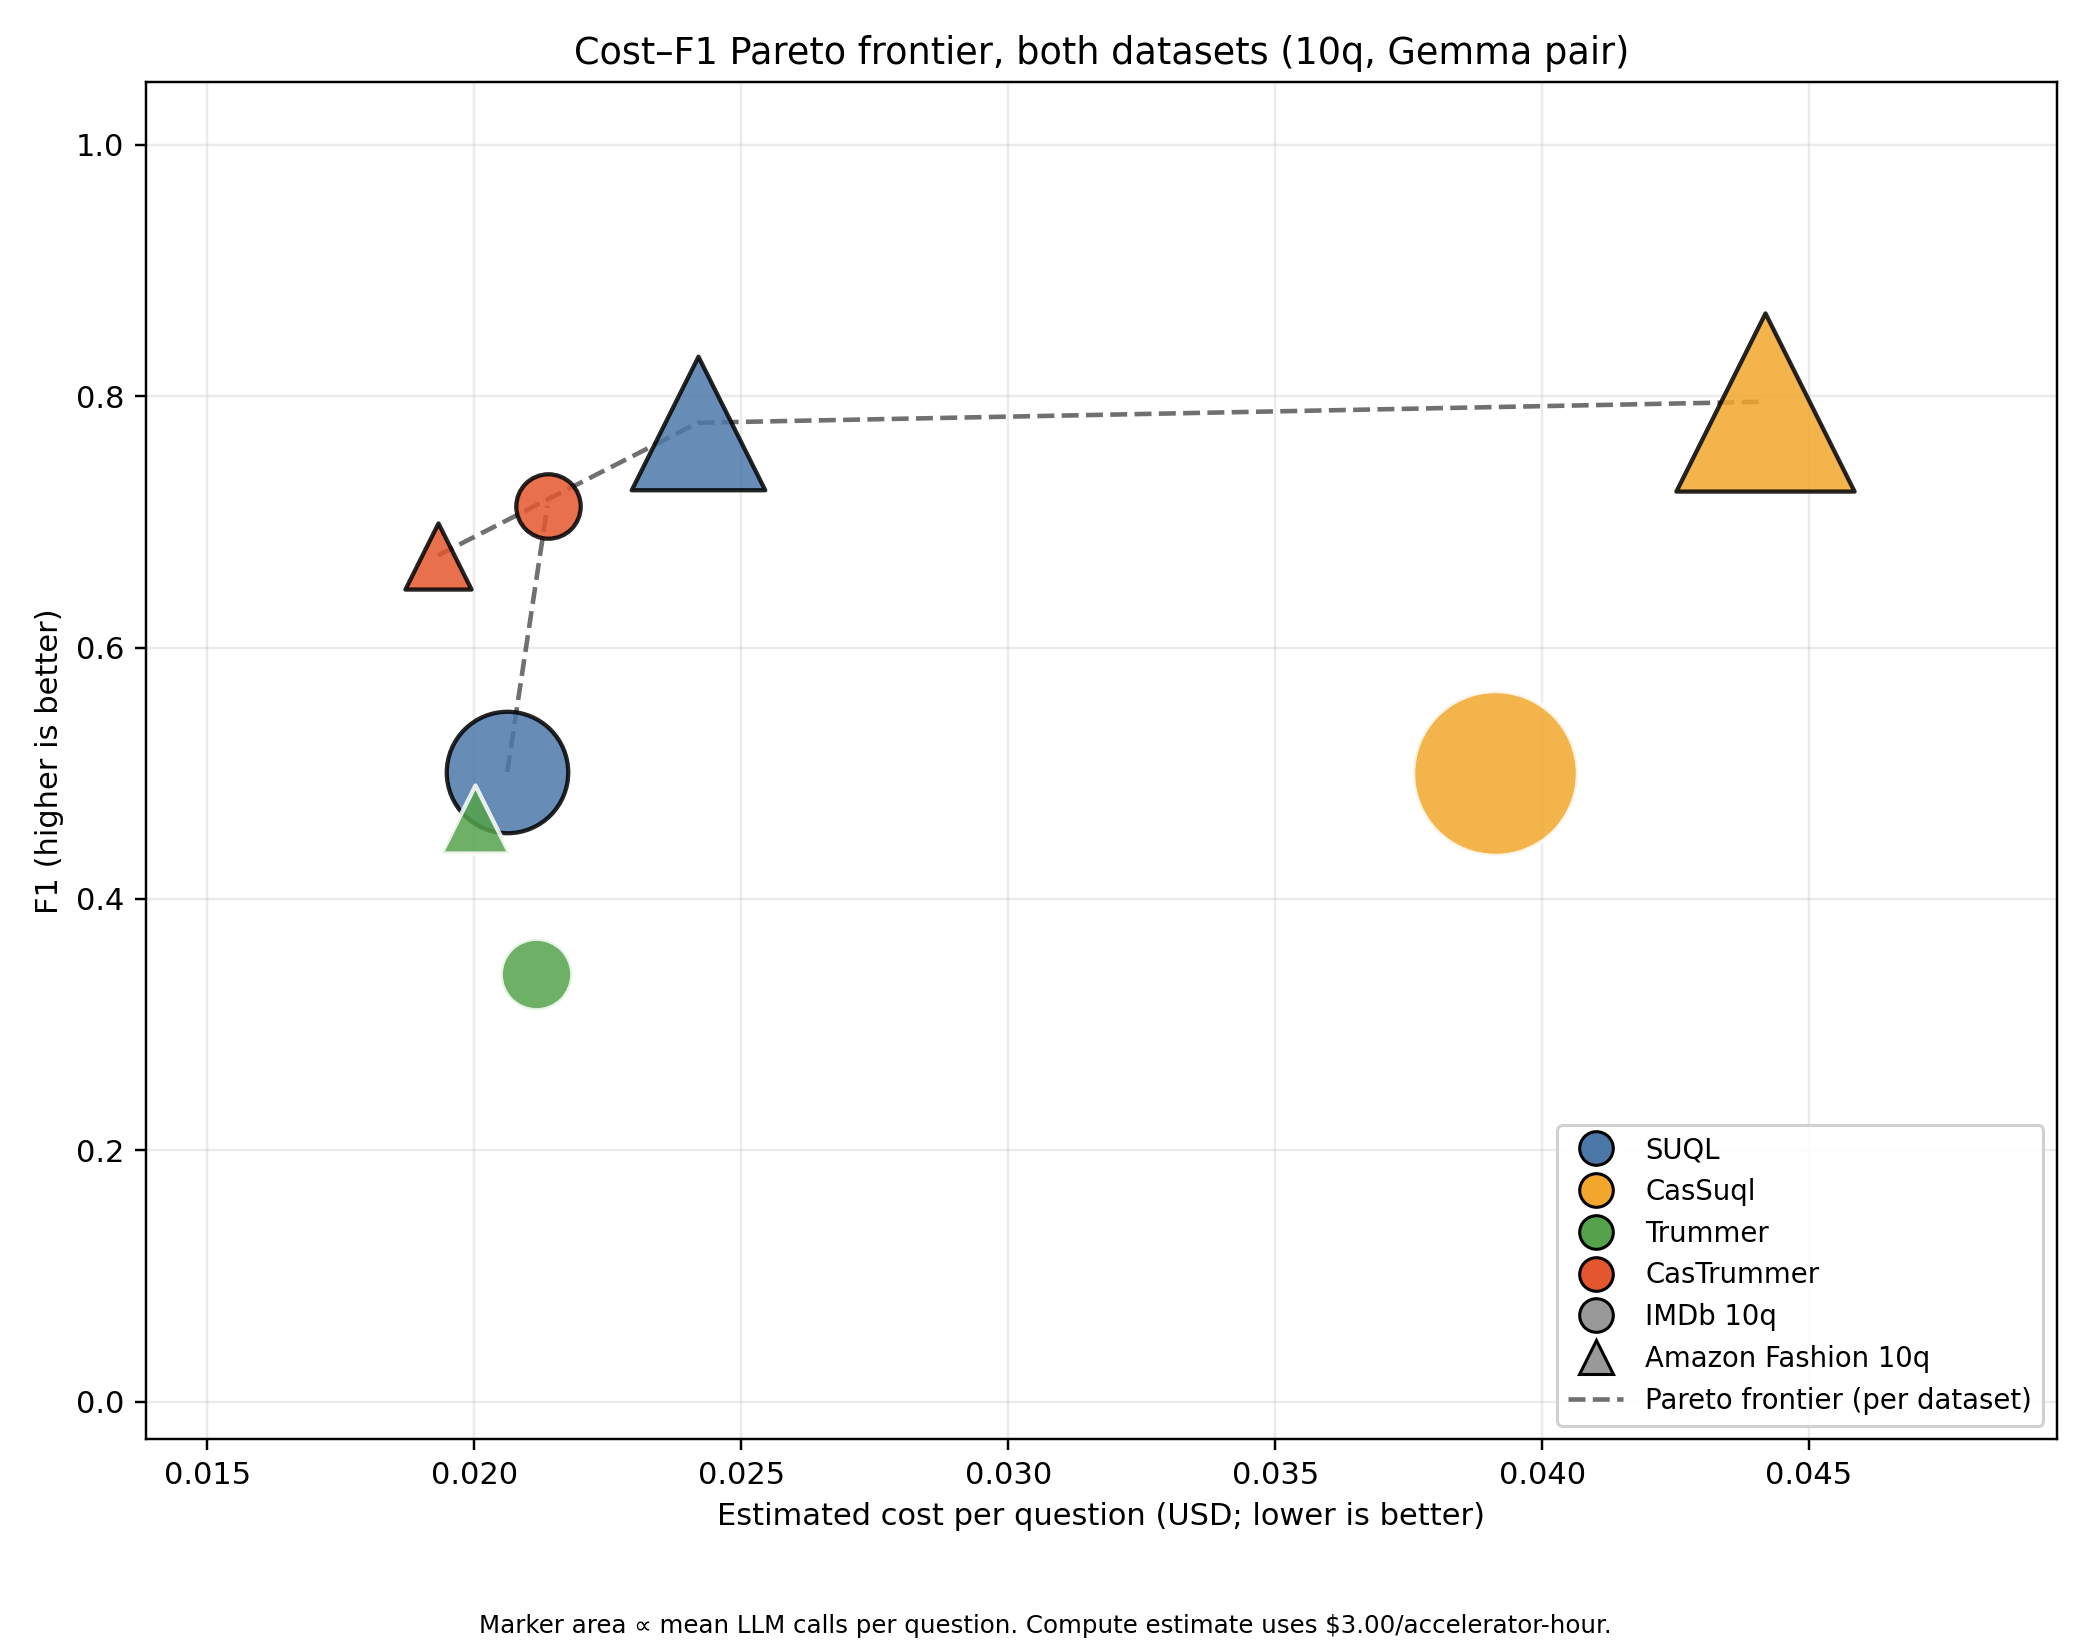
\includegraphics[width=\columnwidth]{figs/pareto/cost_f1_pareto_both_datasets.png}
\caption{Cost--F1 trade-off on \textit{IMDb} (circles) and \textit{Amazon Fashion} (triangles).}
\label{fig:pareto}
\end{figure}

\textbf{Quality.} \textsc{CasTrummer} raises the F1 of \textsc{Trummer} from 0.340 to 0.713 on \textit{IMDb} (+110\%, recall 0.275 to 0.708) and from 0.464 to 0.673 on \textit{Amazon Fashion} (+45\%, mostly through precision, 0.565 to 0.755). The paired gain over the ten questions is $+0.373\pm0.076$ (better on all ten) and $+0.209\pm0.057$ (better on nine), and \textsc{CasTrummer} is the best (or tied best) of the four methods on seven (\textit{IMDb}) and five (\textit{Amazon Fashion}) questions (Table~\ref{tab:perq}). \textsc{CasSuql} reproduces the quality of \textsc{Suql} (F1 0.500 against 0.501, paired difference $-0.001\pm0.022$; 0.796 against 0.779, $+0.017\pm0.015$) with exactly the same recall (0.400; 0.807), and is never more than 0.05 F1 below \textsc{Suql} on eight (\textit{IMDb}) and nine (\textit{Amazon Fashion}) questions.

\textbf{Calls and cost.} \textsc{CasTrummer} issues 81.1\% (\textit{IMDb}) and 83.3\% (\textit{Amazon Fashion}) fewer LLM calls than \textsc{Suql} and 28.0\% and 8.4\% fewer than \textsc{Trummer}. Its wall-clock time equals that of \textsc{Suql} on \textit{IMDb} ($+3.7\%$) and is 20.1\% lower on \textit{Amazon Fashion}, where it is also the cheapest method in dollars ($-20\%$ against \textsc{Suql}). \textsc{CasSuql} sends 5.0\% and 13.8\% fewer rows to the expensive model than \textsc{Suql}. In Figure~\ref{fig:pareto}, \textsc{CasTrummer} and \textsc{Suql} form the Pareto front on both datasets: \textsc{CasTrummer} reaches F1 0.713 against 0.501 on \textit{IMDb} at a cost 4\% higher, and is the cheapest on \textit{Amazon Fashion}, where \textsc{Suql} keeps the higher F1 (0.779 against 0.673).

\textbf{The calibration does what it certifies.} \textsc{CasSuql} certified a reject region in 34\% (\textit{IMDb}) and 77\% (\textit{Amazon Fashion}) of its repetitions, and recall did not drop in any dataset; when the sample cannot certify a band the cascade falls back to the expensive model instead of guessing. \textsc{CasSuql} collapsed on no question (no F1 of 0 where \textsc{Suql} exceeded 0.3), and no row was judged twice.

\textbf{Where the gain comes from, and what the cheap stage costs.} The cheap stage decided on its own only 2.0 of 40 rows (\textit{IMDb}) and 7.4 of 50 (\textit{Amazon Fashion}) for \textsc{CasSuql}, and 1.4 and 0.9 for \textsc{CasTrummer}. Column \textit{CasT$^{-}$} of Table~\ref{tab:results} runs \textsc{CasTrummer} with $|C|{=}0$, so that every row passing $\sigma_S$ is verified by the expensive model in batches. On \textit{IMDb} it is as accurate (F1 0.723 against 0.713; paired difference $-0.010\pm0.035$) and 3.4\,s faster; on \textit{Amazon Fashion} \textsc{CasTrummer} is better by $0.052\pm0.026$ at equal recall, which we cannot separate from an effect of batch partitioning. The quality gain over \textsc{Trummer} (+0.38 and +0.16 without the cheap stage) therefore comes from the other parts of the \textsc{CasTrummer} architecture, structural filtering and batched expensive verification with retry; the calibrated cheap stage adds a recall guarantee without a measurable quality cost, at 1.8--3.4\,s of extra wall-clock time. For \textsc{CasSuql} the cost model of \S\ref{sec:cost} explains the time: a cheap call took 0.58\,s against 0.62\,s for an expensive one on \textit{IMDb} (0.55 against 0.59\,s on \textit{Amazon Fashion}), so $t_c/t_e\approx0.94$ while $d\le0.15$, and \textsc{CasSuql} takes 1.8 to 1.9 times the time of \textsc{Suql}. Stand-alone measurements of other pairs (Table~\ref{tab:pairs}) show wider gaps, down to $t_c/t_e=0.30$ for Llama~3.1 8B and 70B, with cheap scores of comparable quality (AUC 0.81--0.85); there a row-wise cascade would need to decide only about a third of the rows to save time, which our simulations suggest a calibration set of about 40 rows can reach (\S\ref{sec:cascade-math}). We have not yet evaluated these pairs.

\begin{table}[t]
\centering\footnotesize
\setlength{\tabcolsep}{4pt}
\begin{tabular}{llrrrr}
\toprule
Cheap $\to$ expensive & AUC & $t_c$ (s) & $t_e$ (s) & $t_c/t_e$ \\
\midrule
Gemma 4 e2b $\to$ 26b (used here) & 0.85 & 0.42 & 0.65 & 0.65 \\
Gemma 4 e2b $\to$ 31b & 0.85 & 0.42 & 0.79 & 0.54 \\
Qwen 3.5 2b $\to$ 27b & 0.83 & 0.36 & 1.00 & 0.36 \\
Llama 3.1 8b $\to$ 70b & 0.81 & 0.23 & 0.78 & 0.30 \\
\bottomrule
\end{tabular}
\caption{Stand-alone latency of candidate model pairs on \textit{IMDb} rows (single stream, H200): $t_c$ is a one-token scoring call of the cheap model, $t_e$ an answer call of the expensive one; AUC is that of the cheap model's log-odds against the ground truth (120 rows). Only the first pair is evaluated in this paper.}
\label{tab:pairs}
\end{table}

\textbf{Which cascade to use.} \textsc{CasTrummer} is the choice when calls and dollars matter: it improves the F1 of \textsc{Trummer} on nine or ten of the ten questions and issues about 80\% fewer calls than \textsc{Suql}, although on \textit{Amazon Fashion} \textsc{Suql} remains the more accurate. \textsc{CasSuql} is the choice when the quality of row-wise judgments must be preserved with a certified bound on what the cheap stage rejects; it pays a time overhead until the cheap model is much faster than the expensive one.

\textbf{Scope.} We use one model pair, ten questions per dataset, pools of 40 and 50 candidates (so 20 calibration rows are 40--50\% of a pool), and lexical ground truth. On one \textit{Amazon Fashion} question the F1 of \textsc{CasTrummer} is 0, which drives its large deviation.

\section{Conclusion}
\label{sec:conclusion}

\textsc{CasSuql} and \textsc{CasTrummer} run the structured filter in the DBMS and put a cheap stage with a statistically calibrated band in front of the semantic operators of \textsc{Suql} and \textsc{Trummer}. The calibration is valid and conservative, wastes no label, and lets the cascades keep the recall of the expensive model; \textsc{CasTrummer} improves the F1 of \textsc{Trummer} by 45--110\% and issues 81--83\% fewer calls than \textsc{Suql}. The cheap stage saves time only when it is much faster than the expensive one and certified on many rows ($t_c/t_e<d$). Future work targets exactly that regime: model pairs with a larger latency gap, calibration sets that grow with the pool (about 10\% to decide half of it), larger pools, and more than two stages.

\bibliographystyle{ACM-Reference-Format}
\bibliography{refs}
\end{document}
